% !TeX program = pdflatex
% AntiFLipper -- all result tables, figures and in-text numbers are generated by
% make_results.py from the experiment outputs. Run it before compiling.
\documentclass[conference]{IEEEtran}

\usepackage{amsmath,amssymb,amsfonts}
\usepackage{graphicx}
\usepackage{booktabs}
\usepackage{pifont}
\usepackage{url}
\usepackage{tikz}
\usetikzlibrary{arrows.meta,positioning,fit,backgrounds,calc,shapes.geometric,shapes.symbols,shadows}
\usepackage[ruled,vlined,linesnumbered]{algorithm2e}
\usepackage{cite}

\newtheorem{proposition}{Proposition}
% generated by make_results.py -- do not edit
\newcommand{\headAcc}{72.0}
\newcommand{\headAccVone}{71.0}
\newcommand{\headAccFLTrust}{69.2}
\newcommand{\headAccLFighter}{59.0}
\newcommand{\headAccFedAvg}{44.2}
\newcommand{\headAccCR}{70.7}
\newcommand{\headFPRFLTrust}{0.44}
\newcommand{\headFPRVone}{0.08}
\newcommand{\headFPRcc}{0.25}
\newcommand{\headRecallLFighter}{0.46}
\newcommand{\headRecallFLAME}{0.42}
\newcommand{\headDet}{15}
\newcommand{\defMs}{30}
\newcommand{\defMsVone}{23}
\newcommand{\defMsFedAvg}{34}
\newcommand{\defMsFLTrust}{352}
\newcommand{\rootMsFLTrust}{115}
\newcommand{\defMsFLAME}{1058}
\newcommand{\defMsKrum}{875}
\newcommand{\evalOverhead}{6.8}
\newcommand{\cleanHonVone}{18.3}
\newcommand{\cleanHonCR}{0.0}
\newcommand{\cleanHonCROnly}{0.3}
\newcommand{\cleanHonBudget}{8.0}
\newcommand{\cleanHonZthree}{17.7}
\newcommand{\cleanAccVone}{16.3}
\newcommand{\cleanAcc}{54.3}
\newcommand{\cleanAccCROnly}{60.2}
\newcommand{\cleanAccCConly}{57.6}
\newcommand{\cleanAccMid}{66.5}
\newcommand{\cleanAccMidVone}{40.7}
\newcommand{\skewAcc}{49.1}
\newcommand{\skewAccStd}{11.9}
\newcommand{\skewAccFedAvg}{43.8}
\newcommand{\skewAccFedAvgStd}{9.1}
\newcommand{\skewAccLFighter}{41.6}
\newcommand{\skewAccFLTrust}{39.3}
\newcommand{\skewAccVone}{13.0}
\newcommand{\skewRecall}{0.96}
\newcommand{\skewDet}{70}
\newcommand{\fakeRecallVone}{0.67}
\newcommand{\fakeRecallCROnly}{0.62}
\newcommand{\fakeRecall}{1.00}
\newcommand{\fakeAcc}{72.0}
\newcommand{\ratioAccLow}{74.1}
\newcommand{\ratioAccFedAvgLow}{74.3}
\newcommand{\ratioAccThirty}{72.4}
\newcommand{\ratioAccFedAvgThirty}{61.0}
\newcommand{\ratioAccLFighterThirty}{64.9}
\newcommand{\bnsafeHead}{57.8}
\newcommand{\mnistAcc}{98.7}
\newcommand{\nRuns}{315}


\begin{document}

\title{\fontsize{21}{25}\selectfont AntiFLipper: A Secure and Efficient Defense Against\\ Label-Flipping Attacks in Federated Learning}

\author{\IEEEauthorblockN{Aashnan Rahman$^{1}$, Abid Hasan$^{2}$, Sherajul Arifin$^{3}$, Faisal Haque Bappy$^{4}$, Tahrim Hossain$^{5}$,\\ Tariqul Islam$^{6}$, Abu Raihan Mostofa Kamal$^{7}$, and Md. Azam Hossain$^{8}$}
\IEEEauthorblockA{
$^{1, 2, 7, 8}$ Islamic University of Technology, Bangladesh.\\
$^{3}$ United International University, Bangladesh.\\
$^{4, 5, 6}$ University of Maryland, Baltimore County, United States.}
}

\maketitle

\begin{abstract}
In a label-flipping attack, malicious clients in federated learning (FL) train on deliberately mislabeled data. They run the unmodified training code, so their updates are hard to tell apart from those of honest clients whose data are simply skewed. A lightweight countermeasure is accuracy feedback: each client evaluates the global model on its own data, and clients that fit their labels poorly lose trust. We show that this signal fails in two ways. It penalizes honest clients that hold hard classes, and attackers can evade it by reporting the result an honest client would obtain. We present AntiFLipper, which keeps feedback cheap and needs no data at the server. Clients report per-class counts, and the server compares each report with the accuracy expected for that client's label mix. A last-layer consistency check adds a signal taken from the update rather than the report. On CIFAR-10 with strong label skew and no attackers, the number of honest clients wrongly excluded falls from \cleanHonRaw{} to \cleanHon{} of 20. With 40\% attackers that flip all labels and report honestly under moderate skew, AntiFLipper is more accurate than six baselines and excludes every attacker without false positives. In the same setting it also excludes every attacker that flips only part of its labels or fakes its reports. Under strong skew it finds \skewRecall{} of the attackers that report honestly, but against report faking in that setting it detects only \fsFound{} of \fsTotal{} attackers across three seeds. Each report adds 84 bytes per round.
\end{abstract}

\begin{IEEEkeywords}
Federated learning, label flipping, data poisoning, data heterogeneity, malicious client detection.
\end{IEEEkeywords}

% =============================================================================
\section{Introduction}
% =============================================================================
Federated learning (FL) lets many clients, such as phones, sensors and hospitals, train a shared model without sending their data to a central server~\cite{fedavg-pmlr-v54-mcmahan17a,kairouz2021advances}. The server only sees model updates, so it cannot check how those updates were produced. This makes FL vulnerable to data poisoning~\cite{lyu2020threats}. The simplest form is \emph{label flipping}: a malicious client relabels part or all of its data, for example by swapping pairs of classes, and then trains as usual~\cite{biggio2011support,tolpegin2020data}. No change to the protocol or the training code is needed, yet a large enough group of such clients can steer the global model towards systematic misclassification.

Detecting these clients is hard because honest clients also differ. In practice each client holds a different mix of classes, and an honest client with an unusual mix produces an unusual update. Most existing defenses inspect the updates at the server, using robust statistics, distances or clustering~\cite{yin2018byzantine,NIPS2017_f4b9ec30,nguyen2022flame,jebreel2024lfighter}. These methods are costly for large models and can confuse heterogeneous honest clients with attackers~\cite{li2023hscs,shen2024lfrppfl}. Others score each client against a clean dataset held by the server~\cite{cao2020fltrust}, which many deployments do not have.

A cheaper signal comes from the clients themselves. If most clients are honest, the global model learns the true labels and fits a flipper's relabelled data poorly. Each client can therefore evaluate the global model on its own data and report its accuracy, and the server can lower the trust of clients that report poorly. This \emph{accuracy feedback} needs no server data and costs one forward pass per round~\cite{andreina2021baffle,jiang2023dataquality}. The signal is, however, less clean than it appears. An honest client may score low simply because it holds harder classes, and a malicious client can report whatever an honest client would report. Both problems grow with data heterogeneity, which is exactly when a defense is most needed.

This paper presents \textbf{AntiFLipper}, a defense that keeps the low cost of accuracy feedback but addresses both problems. Instead of asking whether a client's accuracy is low, the server asks whether it is lower than \emph{expected for the classes that client holds}. A second, inexpensive check looks at what the client actually sent, so that a convincing report alone is not enough to stay trusted. Our contributions are:
\begin{itemize}
\item An analysis showing that raw accuracy feedback penalizes label mix as well as poisoning, and that no detector based on reports alone can identify a client that fakes its report.
\item AntiFLipper, which combines a \emph{class-conditional residual} computed from per-class report counts with a last-layer \emph{consistency check} of the update, and excludes at most the number of clients the threat model allows.
\item An evaluation on CIFAR-10 and MNIST against six defenses. It covers heterogeneity from mild to strong, 10--40\% attackers, partial flips, report faking, component ablations, parameter sensitivity, and measured client, server and communication cost.
\end{itemize}

Section~\ref{sec:related} reviews related work and the two failure modes of accuracy feedback. Section~\ref{sec:model} states the system and threat model, Section~\ref{sec:design} presents AntiFLipper, and Section~\ref{sec:analysis} analyzes it. Sections~\ref{sec:setup} and~\ref{sec:results} describe the experiments, Section~\ref{sec:limits} discusses limitations, and Section~\ref{sec:conclusion} concludes.

% =============================================================================
\section{Related Work}
\label{sec:related}
% =============================================================================
\textbf{Label-flipping and other poisoning attacks.} Label flipping was first studied as adversarial label noise in centralized learning~\cite{biggio2011support}, and optimized poisoning of deep networks was later shown to be feasible~\cite{munoz2017towards}. Tolpegin et al.~\cite{tolpegin2020data} showed that in FL, flipping the labels of one class can sharply reduce the accuracy on that class even with a minority of malicious clients, and that the damage grows with their share. Lavaur et al.~\cite{lavaur2024systematic} report similar effects for FL-based intrusion detection. Shejwalkar et al.~\cite{shejwalkar2022backdrawingboard} argue that data poisoning is weak in production FL when attackers are very few; our setting, with up to 40\% malicious clients, models a stronger adversary. Model-poisoning attacks that craft updates directly~\cite{fang2020local,shejwalkar2021manipulating} and backdoors~\cite{bagdasaryan2020backdoor,wang2020attack} are a different threat and are outside our scope.

\textbf{Defenses that inspect updates.} Byzantine-robust aggregation limits the influence of outlying updates. Coordinate-wise Median and Trimmed Mean~\cite{yin2018byzantine} aggregate each parameter robustly, Krum and Multi-Krum~\cite{NIPS2017_f4b9ec30} select updates close to their neighbors, and Bulyan~\cite{mhamdi2018hidden} combines both but needs $N\ge4f+3$ clients to tolerate $f$ attackers. FoolsGold~\cite{fung2020limitations} down-weights clients whose update histories are suspiciously similar. FLAME~\cite{nguyen2022flame} clusters updates, clips them and adds noise, and CRFL~\cite{xie2021crfl} certifies robustness against backdoors. Defenses aimed at label flipping look at the output layer, where the attack leaves its clearest trace: Tolpegin et al.~\cite{tolpegin2020data} cluster last-layer updates, and LFighter~\cite{jebreel2024lfighter} clusters the gradients of the output neurons that change most. All of these methods treat dissimilar updates as suspicious. Under non-IID data, honest updates are dissimilar too, which is why heterogeneity remains a central difficulty~\cite{li2020federated,li2023hscs,shen2024lfrppfl}.

\textbf{Defenses that use server data.} FLTrust~\cite{cao2020fltrust} trains a reference update on a small clean dataset at the server and weights each client by its similarity to it. HSCS~\cite{li2023hscs} also relies on a small clean dataset to select clients under non-IID data. Such data may be unavailable or unrepresentative of the clients.

\textbf{Feedback- and trust-based defenses.} A third line of work asks clients for information about their own data. In BaFFLe~\cite{andreina2021baffle}, clients validate each global model on their local data and vote on whether to accept it. Other schemes estimate the quality of each client's labels~\cite{jiang2023dataquality,ovi2023confident}, derive trust from a guiding signal~\cite{li2025flgt}, align client distributions at two granularities~\cite{fedalign2026}, or add a dedicated detection pipeline~\cite{abroshan2025aitoprotect}. LFR-PPFL~\cite{shen2024lfrppfl} protects such statistics cryptographically. These approaches avoid server data but usually treat a low score as evidence of poisoning.

\textbf{Where accuracy feedback fails.} Two failure modes of raw accuracy feedback motivate our design. First, accuracy depends on which classes a client holds. Some classes are harder for the current model than others, so an honest client that holds mostly hard classes reports a low accuracy and is treated like an attacker. With strong skew this can trigger a cascade: excluding such clients removes their classes from training, which makes those classes harder and lowers the reports of the remaining clients that hold them (Fig.~\ref{fig:traj}). Second, a report is only a claim. An attacker can train on flipped labels but evaluate the model on its original labels and report that result, which is exactly what an honest client with the same data would report. No rule that looks only at reports can catch it (Prop.~\ref{prop:faking}).

\textbf{Positioning.} AntiFLipper belongs to the feedback family. It needs no server data, and its report is a few bytes. It differs from prior feedback defenses in two ways: it judges each report against what that client's label mix predicts, and it pairs the report with one cheap statistic of the update itself. Neither part requires clustering or distances between full models.

% =============================================================================
\section{System and Threat Model}
\label{sec:model}
% =============================================================================
\textbf{System.} A server coordinates $N$ clients over $T$ rounds. Client $j$ holds a dataset $D_j$ with labels in $\{1,\dots,K\}$ and label mix $\pi_{jk}=n_{jk}/|D_j|$, where $n_{jk}$ is its number of class-$k$ samples. In round $t$, every client that has not been excluded receives the global model $M_t$, trains it for $E$ local epochs and returns the model $m_{j,t}$. Along with it, the client sends a report: the accuracy $a_j$ of $M_t$ on its local labels, together with its per-class correct counts $\mathbf{c}_j$ and sample counts $\mathbf{n}_j$. The server keeps a trust value $\tau_j$ per client, normalized to sum to one, and a set $\beta$ of excluded clients.

\textbf{Adversary.} The adversary controls a fraction $p\le 0.4$ of the clients. We stay below one half so that coordinate-wise medians remain informative, and evaluate $p\in\{0.1,0.2,0.3,0.4\}$. Malicious clients relabel their data with a fixed permutation $\pi$ ($0{\leftrightarrow}1$, $2{\leftrightarrow}3$, \dots, $8{\leftrightarrow}9$) and run the honest training code. A \emph{full flip} relabels all of a client's samples in every round. A \emph{partial flip} relabels a given fraction of them, drawn afresh at random in each round, so the corrupted subset changes over time. We consider two reporting behaviors:
\begin{itemize}
\item \emph{Honest reporting.} The client reports statistics of $M_t$ on the labels it trains on.
\item \emph{Report faking (adaptive).} The client reports statistics of $M_t$ on its \emph{original} labels, exactly as an honest client with the same data would.
\end{itemize}
Crafted updates such as gradient scaling or backdoors~\cite{bagdasaryan2020backdoor,fang2020local} are outside our scope. They are the domain of Byzantine-robust aggregation, with which AntiFLipper can be combined.

% =============================================================================
\section{AntiFLipper}
\label{sec:design}
% =============================================================================
AntiFLipper addresses the two failure modes with two signals. The class-conditional residual corrects reports for label mix, and the consistency check observes the update instead of the report. Trust, flags and a capped exclusion rule turn both signals into an aggregation decision. Fig.~\ref{fig:arch} shows one round, and Algorithm~\ref{alg:af} lists the server procedure.

\begin{figure}[t]
\centering
\resizebox{\columnwidth}{!}{% AntiFLipper architecture (one round). Included by AntiFlipper_v10.tex.
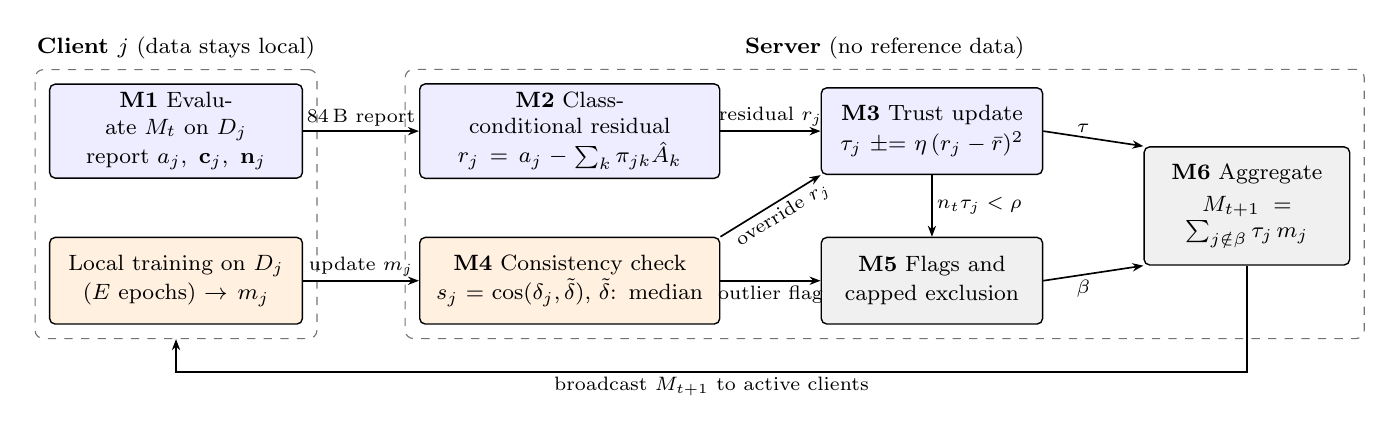
\begin{tikzpicture}[
  font=\footnotesize, >={Stealth[length=4pt]},
  box/.style={draw, rounded corners=2pt, align=center, inner sep=3pt, minimum height=11mm, line width=0.5pt},
  rep/.style={box, fill=blue!7},
  upd/.style={box, fill=orange!12},
  ctl/.style={box, fill=gray!12},
  lab/.style={font=\scriptsize, inner sep=1.5pt},
  flow/.style={->, line width=0.6pt},
]
% ---- clients
\node[rep, text width=3.0cm] (eval)  at (0, 0.95) {\textbf{M1} Evaluate $M_t$ on $D_j$\\[1pt] report $a_j,\ \mathbf{c}_j,\ \mathbf{n}_j$};
\node[upd, text width=3.0cm] (train) at (0,-0.95) {Local training on $D_j$\\[1pt] ($E$ epochs) $\rightarrow m_j$};
\begin{scope}[on background layer]
\node[draw=black!55, dashed, rounded corners=3pt, fit=(eval)(train), inner sep=5pt,
      label={[font=\footnotesize]above:\textbf{Client $j$} (data stays local)}] (clients) {};
\end{scope}

% ---- server
\node[rep, text width=3.6cm] (cr)    at (5.0, 0.95) {\textbf{M2} Class-conditional residual\\[1pt] $r_j = a_j - \sum_k \pi_{jk}\hat A_k$};
\node[upd, text width=3.6cm] (cc)    at (5.0,-0.95) {\textbf{M4} Consistency check\\[1pt] $s_j=\cos(\delta_j,\tilde\delta)$, $\tilde\delta$: median};
\node[rep, text width=2.6cm] (trust) at (9.6, 0.95) {\textbf{M3} Trust update\\[1pt] $\tau_j \mathrel{\pm}= \eta\,(r_j-\bar r)^2$};
\node[ctl, text width=2.6cm] (flag)  at (9.6,-0.95) {\textbf{M5} Flags and\\[1pt] capped exclusion};
\node[ctl, text width=2.4cm, minimum height=15mm] (agg) at (13.6, 0) {\textbf{M6} Aggregate\\[2pt] $M_{t+1}=$\\ $\sum_{j\notin\beta}\tau_j\, m_j$};
\begin{scope}[on background layer]
\node[draw=black!55, dashed, rounded corners=3pt, fit=(cr)(cc)(trust)(flag)(agg), inner sep=5pt,
      label={[font=\footnotesize]above:\textbf{Server} (no reference data)}] (server) {};
\end{scope}

% ---- flows
\draw[flow] (eval)  -- node[lab, above] {84\,B report} (cr);
\draw[flow] (train) -- node[lab, above] {update $m_j$} (cc);
\draw[flow] (cr)    -- node[lab, above] {residual $r_j$} (trust);
\draw[flow] (cc.north east) -- node[lab, sloped, below, pos=0.55] {override $r_j$} (trust.south west);
\draw[flow] (cc)    -- node[lab, below] {outlier flag} (flag);
\draw[flow] (trust) -- node[lab, right] {$n_t\tau_j<\rho$} (flag);
\draw[flow] (trust.east) -- node[lab, above, pos=0.4] {$\tau$} (agg.north west);
\draw[flow] (flag.east)  -- node[lab, below, pos=0.4] {$\beta$} (agg.south west);
\draw[flow] (agg.south) -- ++(0,-1.35) -| node[lab, pos=0.25, below] {broadcast $M_{t+1}$ to active clients} (clients.south);
\end{tikzpicture}
}
\caption{One round of AntiFLipper. Each client sends a short report (blue) and its model update (orange). The server scores reports against each client's label mix, checks updates against the median, and aggregates only trusted clients; an attacker (red) is excluded.}
\label{fig:arch}
\end{figure}

\textbf{M1: Client report.} Before training, client $j$ runs one forward pass of $M_t$ over $D_j$. It records the accuracy $a_j$ and, for every class $k$, the number of correct predictions $c_{jk}$ and of samples $n_{jk}$. With 32-bit values the report payload is $4+8K$ bytes, i.e., 84 bytes for $K{=}10$.

\textbf{M2: Class-conditional residual.} The server pools per-class accuracy over clients, weighted by trust, and compares each report with the accuracy expected for that client's label mix:
\begin{equation}
\hat A_k=\frac{\sum_i \tau_i c_{ik}}{\sum_i \tau_i n_{ik}},\qquad
r_j=a_j-\sum_k \pi_{jk}\hat A_k .
\label{eq:cr}
\end{equation}
Classes with no trust-weighted samples are skipped, and so are classes the client does not hold. An honest client that holds hard classes reports a low $a_j$ but also has a low expectation, so its residual stays close to zero. A flipper fits its own labels poorly in every class it holds, so its residual is expected to be negative, provided that the reference $\hat A_k$ is dominated by honest clients. Because $\hat A_k$ includes the scored client's own report, this condition can fail for a class held mostly by flippers. Section~\ref{sec:analysis} analyzes this bias, and Section~\ref{sec:results} measures the resulting separation.

\textbf{M3: Trust update.} With $\bar r$ the mean residual, trust moves by the squared deviation and is then renormalized over the active clients:
\begin{equation}
\tau_j \leftarrow \max\!\big(0,\ \tau_j + \operatorname{sgn}(r_j-\bar r)\,\eta\,(r_j-\bar r)^2\big).
\label{eq:trust}
\end{equation}
The quadratic form damps small fluctuations and reacts strongly to persistent gaps.

\textbf{M4: Update-consistency check.} Let $\delta_j$ be the change of the classification layer (weights and bias) of client $j$, and $\tilde\delta$ the coordinate-wise median of all $\delta_j$. The server computes $s_j=\cos(\delta_j,\tilde\delta)$ and the robust score $(s_j-\operatorname{med}(s))/(1.4826\,\mathrm{MAD}(s)+\epsilon)$, where $\epsilon{=}10^{-6}$ avoids division by zero when all similarities coincide. A client scoring below $-z$ is \emph{inconsistent}. Its residual is replaced by the round minimum before~(\ref{eq:trust}), and it is flagged in M5.

\textbf{M5: Flags and capped exclusion.} After $g$ warm-up rounds, a client is flagged when $n_t\tau_j<\rho$, i.e., its trust falls below a fixed share of the uniform weight over the $n_t$ active clients, or when M4 marks it inconsistent. Flags accumulate, and a client with $c_{\max}$ flags is excluded. Exclusions are capped at $b=\lfloor0.4N\rfloor$, the bound of the threat model. When more clients qualify, those with the lowest trust are excluded first.

\textbf{M6: Aggregation.} $M_{t+1}=\sum_{j\notin\beta}\tau_j\,m_{j,t}$, with $\tau$ normalized over the active clients.

\setlength{\textfloatsep}{8pt}
\begin{algorithm}[t]
\caption{AntiFLipper: server side of round $t$}
\label{alg:af}
\small
\KwIn{models $m_{j,t}$, reports $(a_j,\mathbf{c}_j,\mathbf{n}_j)$ for $j\notin\beta$; trust $\tau$; flag counts $c$}
$\hat A_k\leftarrow\sum_i\tau_ic_{ik}\,/\sum_i\tau_in_{ik}$ \ for every $k$ with $\sum_i\tau_in_{ik}>0$\;
\lForEach{$j\notin\beta$}{$r_j\leftarrow a_j-\sum_k \pi_{jk}\hat A_k$ \ over the classes defined above, $\pi_j$ renormalized}
$\tilde\delta\leftarrow$ coordinate-wise median of last-layer updates $\{\delta_j\}$\;
$s_j\leftarrow\cos(\delta_j,\tilde\delta)$; \ $I\leftarrow\{j:\ (s_j-\operatorname{med}(s))/(1.4826\,\mathrm{MAD}(s)+\epsilon)<-z\}$\;
\lForEach{$j\in I$}{$r_j\leftarrow\min_i r_i$}
update $\tau$ with~(\ref{eq:trust}) and normalize over $j\notin\beta$\;
\If{$t\ge g$}{
 \ForEach{$j\notin\beta$}{\lIf{$n_t\tau_j<\rho$ \textbf{\upshape or} $j\in I$}{$c_j\leftarrow c_j+1$}}
 $Q\leftarrow\{j\notin\beta:\ c_j\ge c_{\max}\}$ sorted by increasing $\tau_j$\;
 add the first $\max(0,\,b-|\beta|)$ clients of $Q$ to $\beta$; normalize $\tau$\;
}
\Return $M_{t+1}=\sum_{j\notin\beta}\tau_j m_{j,t}$
\end{algorithm}

% =============================================================================
\section{Analysis}
\label{sec:analysis}
% =============================================================================
Let $A_k$ denote the accuracy of $M_t$ on class $k$, and $C_{kl}$ the rate at which it predicts class $l$ for inputs of class $k$. For the following statements we assume that per-class accuracy does not depend on which client a sample comes from, i.e., all clients share $A_k$ and $C_{kl}$.

\begin{proposition}[Raw feedback penalizes label mix]\label{prop:mix}
For an honest client, $\mathbb{E}[a_j]=\sum_k\pi_{jk}A_k$. Its deviation from the population mean is therefore $\sum_k(\pi_{jk}-\bar\pi_k)A_k$, where $\bar\pi_k$ is the population share of class $k$.
\end{proposition}

The deviation is negative whenever a client holds more than its share of hard classes. It vanishes under IID data and is large when each client holds only a few classes, which is the formal counterpart of the first failure mode in Section~\ref{sec:related}.

\begin{proposition}[Residual with exact per-class accuracies]\label{prop:cr}
If $\hat A_k=A_k$ for all $k$, an honest client has $\mathbb{E}[r_j]=0$ for every label mix, while an honestly reporting flipper has $\mathbb{E}[r_j]=-\sum_k\pi_{jk}\,\big(A_{\pi(k)}-C_{k\pi(k)}\big)$.
\end{proposition}
\emph{Proof.} The first claim follows from~(\ref{eq:cr}) and Prop.~\ref{prop:mix}. A flipper's samples of true class $k$ carry label $\pi(k)$. They are counted under $\pi(k)$ and are correct only when $M_t$ predicts $\pi(k)$, at rate $C_{k\pi(k)}$, whereas the expectation uses $A_{\pi(k)}$. \hfill$\square$

In practice $\hat A_k$ is estimated in the presence of flippers. Let $w_k$ be the flippers' trust-weighted share of the samples \emph{labelled} $k$, i.e., their share of $\sum_i\tau_in_{ik}$. Then $\hat A_k$ is biased towards their low class-$k$ accuracy by a factor of up to $w_k$. This share can exceed their overall trust share when flippers hold many samples of class $k$. Because the scored client's own report is part of $\hat A_k$, a single flipper that holds most of a class pulls the reference towards its own accuracy and thereby hides part of its own deficit. The bias lowers every expectation: honest residuals become positive and flipper residuals less negative. Separation therefore requires $w_k$ to remain small, which the trust weighting promotes as flippers lose trust. Prop.~\ref{prop:cr} is thus a statement about the ideal estimate, not a guarantee for every partition.

\begin{proposition}[Report faking defeats report-only detection]\label{prop:faking}
If a flipper reports the statistics of $M_t$ on its original labels, its report has the same distribution as that of an honest client with identically distributed data. No detector that depends only on reports, including the residual, can separate the two better than chance.
\end{proposition}
\emph{Proof.} A faked report is the same function of $(M_t,x,y)$ on the same data distribution as an honest report. The training labels do not enter it. \hfill$\square$

A detector therefore has to observe what a client \emph{did}. Relabelling class $k$ as $\pi(k)$ pushes the classifier row of $\pi(k)$ towards the features of class $k$ and vice versa, which we expect to oppose the last-layer change of honest clients that hold the same classes. With $p<1/2$, every coordinate of $\tilde\delta$ lies between honest values, because the coordinate-wise median has breakdown point $1/2$~\cite{yin2018byzantine}. This bounds the reference vector but does not by itself guarantee that flippers obtain lower cosine similarity than honest clients, whose similarities also spread under heterogeneity. We therefore treat the separation of M4 as an empirical property, use a conservative cut-off ($z{=}3$), and measure its false-positive rate.

\textbf{Exclusion bound.} A client flagged in $c_{\max}$ rounds after warm-up is excluded by its $c_{\max}$-th flagged round unless the cap has been reached. The cap guarantees that at least $0.6N$ clients remain, so no sequence of false positives can empty the federation. We do not claim a convergence guarantee. Even with fixed membership, the trust weights in M6 keep changing, so standard FedAvg analyses~\cite{li2020convergence} do not apply directly. We report training trajectories instead (Fig.~\ref{fig:traj}).

\textbf{Complexity.} The report adds one forward pass over $D_j$ to $E$ training epochs, a relative client cost of roughly $1/(3E)$. On the server, M2 costs $O(n_tK)$, and M4 costs $O(n_t d_L)$ for a last layer of $d_L$ parameters (5{,}130 for ResNet-18 on CIFAR-10). Multi-Krum costs $O(n_t^2W)$ for a $W$-parameter model, FLAME clusters $n_t^2$ similarities in dimension $W$, and FLTrust trains a model on server data every round.

\textbf{Privacy.} Per-class counts reveal a client's label histogram, which a single accuracy value does not. The server, however, needs only the pooled sums in~(\ref{eq:cr}) and one residual per client. The sums $\sum_i\tau_ic_{ik}$ and $\sum_i\tau_in_{ik}$ could be computed with secure aggregation, after which each client derives $r_j$ locally from the broadcast $\hat A$. The server would then again observe one scalar per client. We have not implemented this variant.

% =============================================================================
\section{Experimental Setup}
\label{sec:setup}
% =============================================================================
\textbf{Datasets and models.} CIFAR-10~\cite{CIFAR-krizhevsky2009learning} is trained with ResNet-18~\cite{resnet-he2016deep} (11.2\,M parameters) over 20 clients and 100 rounds. MNIST~\cite{MNIST-lecun1998gradient} is trained with a CNN of 21.8\,k parameters over 100 clients and 200 rounds. The number of clients is the same for IID and non-IID splits. Non-IID splits divide the samples of each class among the clients in proportions drawn from a Dirichlet distribution $\mathrm{Dir}(\alpha_D)$~\cite{ferguson1973bayesian}, with $\alpha_D{=}1$ (moderate skew) unless stated otherwise; $\alpha_D{=}0.1$ gives strong skew. This split also makes client datasets unequal in size. On CIFAR-10 they range from \sizeHighMin{} to \sizeHighMax{} samples at $\alpha_D{=}1$ and from \sizeLowMin{} to \sizeLowMax{} at $\alpha_D{=}0.1$. All clients participate in every round and train for $E{=}3$ epochs with SGD (learning rate 0.01, momentum 0.9, weight decay $5\cdot10^{-4}$, batch size 32 for CIFAR-10 and 64 for MNIST).

\textbf{Attacks.} Unless stated otherwise, 40\% of the clients perform a full flip in every round and report honestly. We use 40\% as the default because it is the largest share our threat model allows and therefore the hardest case: it is where undefended training and several baselines break down (Fig.~\ref{fig:ratio}). We additionally evaluate partial flips of 50\% and 25\% of each attacker's samples, report faking at $\alpha_D{=}1$ and $\alpha_D{=}0.1$, attacker shares of 10--30\%, and runs without attackers, in which every exclusion is a false positive.

\textbf{Baselines.} We compare with FedAvg, coordinate-wise Median, Multi-Krum ($f=\lfloor pN\rfloor$), FLAME, LFighter and FLTrust. FLTrust additionally receives a class-balanced root set of 100 clean samples. Its reference implementation rescales all tensors, including BatchNorm statistics; because this is an implementation choice, we also report a variant that rescales only trainable parameters. Ablations replace the residual with the raw report $a_j$, remove CC or the cap, or use CC alone with uniform trust. All methods share the same partitions and attacker sets. Throughout, FedAvg denotes averaging with equal client weights, not the sample-weighted average of the original algorithm~\cite{fedavg-pmlr-v54-mcmahan17a}. This matches AntiFLipper, whose trust also starts uniform and ignores dataset size, so the two differ only in the defense.

\textbf{Parameters and metrics.} AntiFLipper uses $\eta{=}0.1$, $\rho{=}0.05$, $c_{\max}{=}6$, $g{=}2$, $z{=}3$ and $b{=}0.4N$. Results are means (with standard deviations) over three independent seeds, \nRuns{} training runs in total; the sensitivity study uses separate held-out seeds. Accuracy and attack success rate (ASR, the share of test predictions equal to $\pi(y)$) are averaged over the last 10 rounds, because single rounds fluctuate by several points under strong skew; where it matters, we also report final-round accuracy. Precision, recall and false-positive rate (FPR) refer to the clients that are excluded, or given zero weight by baselines, in the final round. Server time covers all checks, trust updates and aggregation. We report it per training round, excluding rounds known to have overlapped other workloads on the machine, and in a matched benchmark that gives every method the same 20 updates.

% =============================================================================
\section{Results}
\label{sec:results}
% =============================================================================
We first compare AntiFLipper with existing defenses in the standard setting, then examine the two failure modes in turn: honest clients under strong skew, and attackers that try to stay hidden. An ablation then shows which component is responsible for each result.

\begin{table*}[t]
\centering
\caption{Comparison with existing defenses under 40\% label-flipping clients (mean$\pm$std over three seeds).}
\label{tab:main}
\footnotesize
\setlength{\tabcolsep}{4.5pt}
\begin{tabular}{@{}l ccccc c cc@{}}
\toprule
& \multicolumn{5}{c}{\textbf{CIFAR-10, non-IID} ($\alpha_D{=}1$)} & \textbf{CIFAR-10} & \multicolumn{2}{c}{\textbf{MNIST}} \\
\cmidrule(lr){2-6}\cmidrule(lr){7-7}\cmidrule(lr){8-9}
\textbf{Method} & Acc.\,(\%)\,$\uparrow$ & ASR\,(\%)\,$\downarrow$ & Prec.\,$\uparrow$ & Rec.\,$\uparrow$ & FPR\,$\downarrow$ & IID Acc. & non-IID Acc. & IID Acc. \\
\midrule
FedAvg & 44.2{\scriptsize$\pm$0.5} & 32.8 & n/a & n/a & n/a & 42.1{\scriptsize$\pm$0.1} & 49.8{\scriptsize$\pm$0.3} & 49.6{\scriptsize$\pm$0.1} \\
Median & 57.9{\scriptsize$\pm$4.2} & 16.7 & n/a & n/a & n/a & 62.9{\scriptsize$\pm$1.4} & -- & -- \\
Multi-Krum & 60.8{\scriptsize$\pm$15.8} & 12.5 & 0.60 & 0.75 & 0.33 & 72.9{\scriptsize$\pm$0.3} & -- & -- \\
FLAME & 56.9{\scriptsize$\pm$7.7} & 17.7 & 0.49 & 0.42 & 0.17 & 71.1{\scriptsize$\pm$0.4} & -- & -- \\
LFighter & 59.0{\scriptsize$\pm$13.3} & 15.2 & 0.71 & 0.46 & 0.08 & 73.2{\scriptsize$\pm$0.3} & 98.5{\scriptsize$\pm$0.2} & \textbf{98.7}{\scriptsize$\pm$0.1} \\
FLTrust (reference)$^{\dagger}$ & 69.2{\scriptsize$\pm$1.1} & 5.2 & 0.60 & 0.92 & 0.44 & 63.1{\scriptsize$\pm$0.3} & 97.2{\scriptsize$\pm$0.1} & 97.5{\scriptsize$\pm$0.1} \\
FLTrust (BN-safe)$^{\dagger}$ & 57.8{\scriptsize$\pm$1.2} & 15.1 & 0.23 & 0.29 & 0.33 & 63.9{\scriptsize$\pm$2.3} & -- & -- \\
\midrule
\textbf{AntiFLipper} & \textbf{72.0}{\scriptsize$\pm$0.6} & \textbf{3.2} & \textbf{1.00} & \textbf{1.00} & \textbf{0.00} & \textbf{73.3}{\scriptsize$\pm$0.4} & \textbf{98.7}{\scriptsize$\pm$0.1} & \textbf{98.7}{\scriptsize$\pm$0.2} \\
\bottomrule
\end{tabular}
\\[2pt]\parbox{\linewidth}{\scriptsize $^{\dagger}$Uses a 100-sample clean root dataset at the server. Reference: rescales all tensors including BatchNorm statistics; BN-safe: trainable parameters only.}
\end{table*}

\begin{table*}[t]
\centering
\caption{Ablation on CIFAR-10. Each component is added to or removed from AntiFLipper.}
\label{tab:ablation}
\footnotesize
\setlength{\tabcolsep}{4.5pt}
\begin{tabular}{@{}l ccc cc cc cc cc@{}}
\toprule
& & & & \multicolumn{2}{c}{\textbf{40\% attack}} & \multicolumn{2}{c}{\textbf{40\% report-faking}} & \multicolumn{2}{c}{\textbf{No attack}} & \multicolumn{2}{c}{\textbf{40\% attack}} \\
& & & & \multicolumn{2}{c}{$\alpha_D{=}1$} & \multicolumn{2}{c}{$\alpha_D{=}1$} & \multicolumn{2}{c}{$\alpha_D{=}0.1$} & \multicolumn{2}{c}{$\alpha_D{=}0.1$} \\
\cmidrule(lr){5-6}\cmidrule(lr){7-8}\cmidrule(lr){9-10}\cmidrule(lr){11-12}
\textbf{Variant} & CR & CC & Cap & Acc. & FPR & Acc. & Rec. & Acc. & Excl.\,$\downarrow$ & Acc. & Rec. \\
\midrule
Raw reports & \ding{55} & \ding{55} & \ding{55} & 71.0 & 0.08 & 72.4 & 0.67 & 16.3 & 18.3 & 13.0 & 0.88 \\
Raw reports + cap & \ding{55} & \ding{55} & \ding{51} & -- & -- & -- & -- & 16.8 & 8.0 & 12.5 & 0.38 \\
Raw reports + CC & \ding{55} & \ding{51} & \ding{55} & 70.4 & 0.25 & 71.6 & 0.88 & 31.2 & 17.0 & 28.9 & \textbf{0.96} \\
CC only & -- & \ding{51} & \ding{55} & 71.4 & 0.11 & 71.4 & \textbf{1.00} & 57.6 & 1.0 & 43.2 & 0.04 \\
CR + cap (no CC) & \ding{51} & \ding{55} & \ding{51} & 70.7 & \textbf{0.00} & \textbf{73.5} & 0.62 & \textbf{60.2} & 0.3 & \textbf{49.1} & \textbf{0.96} \\
\midrule
\textbf{AntiFLipper} & \ding{51} & \ding{51} & \ding{51} & \textbf{72.0} & \textbf{0.00} & 72.0 & \textbf{1.00} & 54.3 & \textbf{0.0} & \textbf{49.1} & \textbf{0.96} \\
\bottomrule
\end{tabular}
\end{table*}


\subsection{Comparison with existing defenses}
Table~\ref{tab:main} gives the main comparison. On CIFAR-10 non-IID with 40\% attackers, AntiFLipper reaches \headAcc\% accuracy, the highest of all methods, and lowers the ASR from \headASRFedAvg\% under FedAvg to \headASR\%. In every seed it excludes all attackers, on average by round \headDet, and no honest client. The reference FLTrust is the strongest baseline at \headAccFLTrust\%, but it flags \headFPRFLTrust{} of the honest clients, relies on server data, and produced non-finite losses in \fltrustNanRounds{} rounds across \fltrustNanRuns{} of its 3 runs. Its BatchNorm-safe variant has no such failures but reaches only \bnsafeHead\%. LFighter and FLAME recover \headRecallLFighter{} and \headRecallFLAME{} of the attackers, and their accuracy, like that of Multi-Krum ($\pm$\headAccKrumStd), varies strongly across seeds. On CIFAR-10 IID and on MNIST, where heterogeneity is mild or absent, the strong methods lie within a fraction of a point of one another, so the differences that matter appear only with skewed data.

\subsection{Honest clients under strong skew}
\begin{figure}[t]
\centering
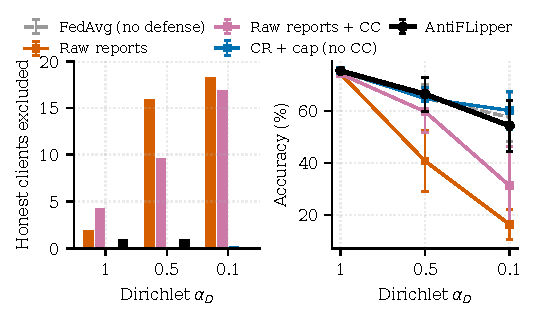
\includegraphics[width=\columnwidth]{fig/gen_heterogeneity.pdf}
\caption{No attackers: honest clients excluded (left) and accuracy (right) on CIFAR-10 as data become more skewed.}
\label{fig:het}
\end{figure}

\begin{figure}[t]
\centering
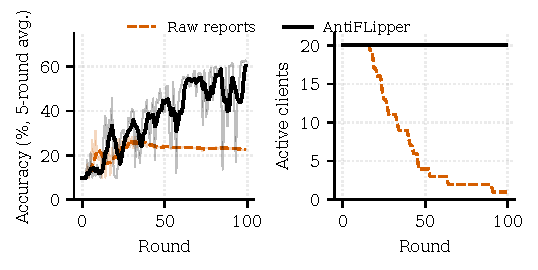
\includegraphics[width=\columnwidth]{fig/gen_trajectories.pdf}
\caption{One run without attackers at $\alpha_D{=}0.1$ (seed \trajSeed, the middle of our three seeds, chosen by seed number rather than by outcome): raw reports exclude honest clients in a cascade; AntiFLipper excludes none.}
\label{fig:traj}
\end{figure}

Fig.~\ref{fig:het} removes the attackers, so every exclusion is a false positive. Raw reports already exclude \cleanHonMidRaw{} of 20 honest clients at $\alpha_D{=}0.5$ and \cleanHonRaw{} at $\alpha_D{=}0.1$, and accuracy collapses to \cleanAccRaw\%. Fig.~\ref{fig:traj} shows how this happens: exclusions accumulate round after round, as predicted in Section~\ref{sec:related}. With the residual, exclusions stay near zero at every level of skew, and accuracy at $\alpha_D{=}0.5$ rises from \cleanAccMidRaw\% to \cleanAccMid\%.

The undefended FedAvg curve in Fig.~\ref{fig:het} is the reference for what is achievable. At $\alpha_D{=}0.1$ it averages \fedCleanAcc$\pm$\fedCleanStd\% over the last 10 rounds and \fedCleanFinal\% in the final round, so training at this level of skew is unstable even without any defense. AntiFLipper averages \cleanAcc$\pm$\cleanAccStd\%, within one standard deviation of FedAvg, and the residual alone \cleanAccCROnly$\pm$\cleanAccCROnlyStd\% (Table~\ref{tab:ablation}). The consistency check marked a client inconsistent in only \ccOverrideShare\% of client-rounds, so these differences do not stem from exclusions. The residual thus removes the penalty of raw feedback; it does not make strongly skewed training more accurate than undefended training.

\subsection{Attackers under strong skew}
\begin{table}[t]
\centering
\caption{Strong heterogeneity: CIFAR-10, $\alpha_D{=}0.1$, 40\% attackers.}
\label{tab:skew}
\footnotesize
\setlength{\tabcolsep}{4.5pt}
\begin{tabular}{@{}l cccc@{}}
\toprule
\textbf{Method} & Acc.\,(\%) & Rec. & FPR & All found \\
\midrule
FedAvg & 43.8{\scriptsize$\pm$9.1} & n/a & n/a & n/a \\
LFighter & 41.6{\scriptsize$\pm$11.5} & 0.21 & 0.28 & n/a \\
FLTrust$^{\dagger}$ & 39.3{\scriptsize$\pm$6.5} & 0.58 & 0.53 & n/a \\
\midrule
Raw reports & 13.0{\scriptsize$\pm$2.6} & 0.88 & 0.94 & 0/3 \\
\textbf{AntiFLipper} & \textbf{49.1}{\scriptsize$\pm$11.9} & \textbf{0.96} & \textbf{0.00} & 2/3 (70) \\
\bottomrule
\end{tabular}
\\[2pt]\parbox{\linewidth}{\scriptsize All found: seeds in which every attacker was excluded (mean round).}
\end{table}

Table~\ref{tab:skew} combines strong skew with 40\% attackers, the hardest setting with honest reporting. AntiFLipper reaches \skewAcc\%, compared with \skewAccFedAvg\% for FedAvg, \skewAccLFighter\% for LFighter and \skewAccFLTrust\% for FLTrust. It finds \skewRecall{} of the attackers without excluding an honest client, whereas raw reports flag \skewFPRRaw{} of the honest clients. Detection is slower and not always complete: all attackers were excluded in \skewFull{} seeds, on average by round \skewDetHits, and in the remaining seed \skewMissed{} attacker was never excluded. Variance across seeds is high for every method in this setting. The per-client logs are consistent with weaker residual separation. We consider the clients that are still active and that the consistency check has not marked. In each of the first ten rounds, we compute the probability that a random attacker among them has a lower residual than a random honest one, and we average over the rounds. This probability is \aucHighMin--\aucHighMax{} per seed at $\alpha_D{=}1$ but only \aucLowMin--\aucLowMax{} at $\alpha_D{=}0.1$. Under strong skew, the residual therefore separates the two groups only weakly, in line with the estimation bias discussed in Section~\ref{sec:analysis}.

\subsection{Attackers that try to stay hidden}
\begin{table}[t]
\centering
\caption{Report-faking attacker (CIFAR-10 non-IID, 40\%): attackers train on flipped labels but report the statistics of their clean labels. Methods that ignore reports are unaffected, so their honest-report runs apply to both columns.}
\label{tab:adaptive}
\renewcommand{\arraystretch}{1.1}
\footnotesize
\setlength{\tabcolsep}{3.5pt}
\begin{tabular}{l|cc|ccc}
\hline
& \multicolumn{2}{c|}{\textbf{Honest reports}} & \multicolumn{3}{c}{\textbf{Faked reports}} \\
\textbf{Method} & Acc. & R & Acc. & R & FPR \\
\hline
LFighter & 59.0$\pm$13.3 & 0.46 & 59.0$\pm$13.3 & 0.46 & 0.08 \\
FLTrust$^\dagger$ & 69.2$\pm$1.1 & 0.92 & 69.2$\pm$1.1 & 0.92 & 0.44 \\
\quad CC only (no reports) & 71.4$\pm$0.3 & 1.00 & 71.4$\pm$0.3 & 1.00 & 0.11 \\
AntiFLipper-v1 (raw reports) & 71.0$\pm$0.2 & 1.00 & 72.4$\pm$0.2 & 0.67 & 0.08 \\
\quad v1 + CC & 70.4$\pm$0.5 & 1.00 & 71.6$\pm$0.5 & 0.88 & 0.17 \\
\quad CR only (no CC) & 70.7$\pm$1.1 & 1.00 & 73.5$\pm$0.8 & 0.62 & 0.00 \\
\textbf{AntiFLipper (CR+CC)} & 72.0$\pm$0.6 & 1.00 & 72.0$\pm$0.3 & 1.00 & 0.00 \\
\hline
\end{tabular}
\end{table}

Table~\ref{tab:adaptive} considers attackers that weaken or disguise their signal. With partial flips, each attacker leaves part of its data untouched and therefore reports a higher accuracy. At the two tested fractions, AntiFLipper still excludes every attacker without false positives, by round \pfDetHalf{} when half of the labels are flipped and by round \pfDetQuarter{} when a quarter are, and its accuracy is \pfAccHalf\% and \pfAccQuarter\%. Weaker attacks thus take longer to detect but were not missed. We did not run the baselines with partial flips, so these rows show detection rather than an accuracy advantage.

Report faking at $\alpha_D{=}1$ is also fully detected, by round \fakeDet{} on average, with no false positives. Raw feedback identifies only \fakeRecallRaw{} of the fakers and the residual alone \fakeRecallCROnly, as Prop.~\ref{prop:faking} predicts, so it is the consistency check that catches them. Under strong skew, however, report faking succeeds: AntiFLipper finds \fsRecall{} of the attackers, and its accuracy (\fsAcc\%) is no better than that of FedAvg (\fsAccFedAvg\%). Here the residual is blind by construction, and the consistency check cannot separate attackers from honest clients whose updates already differ widely. Neither component alone does better: the residual alone finds \fsRecallCR{} of the attackers and the consistency check alone \ccSkewRecall{} (last rows of Table~\ref{tab:adaptive}). This combination is the main open case for AntiFLipper.

\subsection{Ablation}
Table~\ref{tab:ablation} shows which component is responsible for these results. In the main setting all variants perform similarly, and the consistency check alone (with the same $z$ and cap) is as accurate as AntiFLipper (\ccHeadAcc\%). The differences appear in the harder settings. Raw reports fail without attackers under strong skew and against report faking. The cap alone limits the damage (\cleanHonBudget{} honest clients excluded instead of \cleanHonRaw) but does not prevent it. The residual prevents these exclusions in our runs and is what finds attackers under strong skew, but it misses fakers. The consistency check alone catches every faker but finds only \ccSkewRecall{} of the attackers under strong skew, where its accuracy (\ccSkewAcc\%) matches undefended FedAvg. Each signal therefore covers the failure of the other. AntiFLipper is the only variant that excludes no honest client without attackers, catches every faker, and keeps the best recall under strong skew. This shows that the components are complementary, not that both are needed in every single setting; the residual alone, for instance, is more accurate without attackers under strong skew.

\subsection{Share of malicious clients}
\begin{figure}[t]
\centering
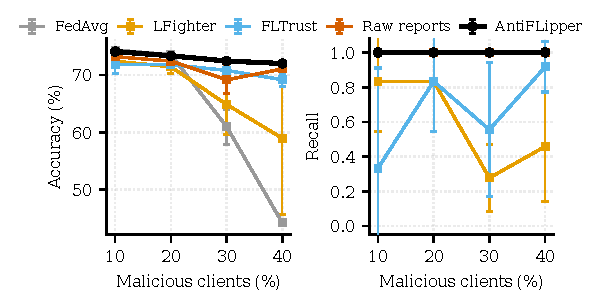
\includegraphics[width=\columnwidth]{fig/gen_ratio.pdf}
\caption{Accuracy and recall on CIFAR-10 non-IID versus the share of malicious clients.}
\label{fig:ratio}
\end{figure}
Fig.~\ref{fig:ratio} varies the share of attackers from 10\% to 40\%. AntiFLipper keeps a recall of 1.0 throughout, with an FPR of at most \ratioFPRmax{} (one or two honest clients in some seeds). At 10\% it matches undefended FedAvg (\ratioAccLow\% vs.\ \ratioAccFedAvgLow\%), so the defense costs nothing when the attack is weak. At 30\% it reaches \ratioAccThirty\%, while FedAvg drops to \ratioAccFedAvgThirty\%, LFighter to \ratioAccLFighterThirty\% and FLTrust to \ratioAccFLTrustThirty\%.

\subsection{Cost and sensitivity}
\begin{table}[t]
\centering
\caption{Cost per round on CIFAR-10 (ResNet-18, 20 clients).}
\label{tab:cost}
\footnotesize
\setlength{\tabcolsep}{3.2pt}
\begin{tabular}{@{}l ccccc@{}}
\toprule
& \textbf{Server} & \multicolumn{2}{c}{\textbf{Server time (ms)}} & \textbf{Client} & \textbf{Report} \\
\cmidrule(lr){3-4}
\textbf{Method} & \textbf{data} & matched & in training & \textbf{overhead} & \textbf{payload} \\
\midrule
FedAvg & \ding{55} & 183 & 34 & 0 & 0 \\
Multi-Krum & \ding{55} & 4109 & 875 & 0 & 0 \\
FLAME & \ding{55} & 3465 & 1058 & 0 & 0 \\
LFighter & \ding{55} & 214 & 42 & 0 & 0 \\
FLTrust$^{\dagger}$ & \ding{51} & 1269 & 352 + 115 & 0 & 0 \\
\midrule
\textbf{AntiFLipper} & \ding{55} & 173 & 30 & 6.8\% & 84\,B \\
\bottomrule
\end{tabular}
\\[2pt]\parbox{\linewidth}{\scriptsize Matched: identical 20 updates on one CPU (Intel i7-8700, 6 threads, PyTorch 2.8), mean of 5 timed iterations after one warm-up; standard deviation 8\,ms for AntiFLipper and 25\,ms for FedAvg. In training: measured per round on an RTX 3090 GPU; excluded clients are not averaged. FLTrust: aggregation + root training.}
\end{table}

\begin{table}[t]
\centering
\caption{One-factor sensitivity of the shared trust/counter/consistency pipeline (v1 + CC, MNIST non-IID, held-out seeds 101, 113, 127). Attack: 40\% flippers. Clean: no attackers, so every exclusion is a false positive.}
\label{tab:sensitivity}
\renewcommand{\arraystretch}{1.1}
\footnotesize
\begin{tabular}{l|cc|c}
\hline
& \multicolumn{2}{c|}{\textbf{Attack}} & \textbf{Clean} \\
\textbf{Setting} & Acc. (\%) & R & FPR \\
\hline
default ($\rho{=}0.05$, $c_{\max}{=}6$, $z{=}2.5$) & 98.6$\pm$0.2 & 1.00 & 0.130 \\
$\rho=0.025$ & 98.6$\pm$0.2 & 1.00 & 0.127 \\
$\rho=0.1$ & 98.6$\pm$0.2 & 1.00 & 0.130 \\
$c_{\max}=3$ & 98.5$\pm$0.2 & 1.00 & 0.323 \\
$c_{\max}=9$ & 98.6$\pm$0.2 & 1.00 & 0.090 \\
$z=2.0$ & 98.5$\pm$0.2 & 1.00 & 0.470 \\
$z=3.0$ & 98.6$\pm$0.2 & 1.00 & 0.050 \\
\hline
\end{tabular}
\end{table}

Table~\ref{tab:cost} reports cost. In the matched benchmark (20 identical updates, CPU), AntiFLipper's server work takes \matchedOurs\,ms, comparable to FedAvg (\matchedFedAvg\,ms) in this benchmark, against \matchedFLTrust\,ms for FLTrust without root training, \matchedKrum\,ms for Multi-Krum and \matchedFLAME\,ms for FLAME. During training we observed \defMs\,ms per round, versus \defMsFedAvg\,ms for FedAvg; these times are not matched, because AntiFLipper averages fewer models once attackers are excluded. The client evaluation adds \evalOverhead\% to local training, and the 84-byte report is negligible next to the 44.7\,MB model update.

Table~\ref{tab:sensitivity} varies the flag limit $c_{\max}$ and the consistency cut-off $z$ on held-out seeds. Accuracy and recall do not change, and recall stays at least \sensRecallMin. Only the FPR without attackers reacts to the most aggressive settings, reaching \sensFPRmax{} in a single run, which motivates the defaults $c_{\max}{=}6$ and $z{=}3$. In an earlier study with raw reports, halving or doubling the trust threshold $\rho$ changed neither accuracy nor recall. MNIST is an easy task, so this study shows robustness to the parameters rather than to the data.

% =============================================================================
\section{Discussion and Limitations}
\label{sec:limits}
% =============================================================================
AntiFLipper's main limitation is the case it does not solve: against attackers that fake their reports under strong skew, AntiFLipper detects only \fsFound{} of \fsTotal{} attackers across three seeds, because the residual cannot see faking and honest updates are too diverse for the consistency check. An attacker that also aligns its last-layer update with the median could evade the check even under mild skew, and we did not evaluate colluding attackers. Under strong skew with honest reporting, detection was incomplete in one of three runs. We have no convergence guarantee, and per-class counts reveal label histograms unless the secure-aggregation variant of Section~\ref{sec:analysis} is deployed, which we have not implemented. Our experiments cover image classification with synchronous full participation; client dropout, partial participation and other data domains remain to be tested. All averaging, in FedAvg and in AntiFLipper, uses equal client weights; we did not evaluate sample-weighted aggregation, which changes the influence of large clients under strong skew. Three seeds support means and standard deviations but not fine-grained significance claims.

% =============================================================================
\section{Conclusion}
\label{sec:conclusion}
% =============================================================================
Accuracy feedback is a cheap and data-free signal against label flipping, but used raw it mistakes skewed honest clients for attackers and can be faked. AntiFLipper judges each report against the client's own label mix and checks the update itself. In our clean CIFAR-10 runs at $\alpha_D{=}0.1$, this reduced the honest clients wrongly excluded from \cleanHonRaw{} of 20 to zero. Under moderate skew it gives the most accurate result among the evaluated defenses with complete and false-positive-free detection, and in that setting it also detects every attacker that flips part of its labels or fakes its reports. Its server time is comparable to that of FedAvg. Report faking under strong skew remains open, as do colluding attackers, the secure-aggregation report and a convergence analysis.

\bibliographystyle{IEEEtran}
\bibliography{IEEEabrv,bibliography_updated}
\end{document}
